\section{Fundamentação Teórica} \label{sec:fundaments}

Para o roteamento de fibras, é necessário pelo menos o entendimento básico de 
dois temas: (1) os elementos que compoem essas redes e (2) algoritmos, no sentido
de operações, otimização e tipos de problemas.

\subsection{Redes Ópticas}

Na teoria dos grafos, um grafo é uma estrutura composta por vértices ($V$)
(também chamados de nós) e arestas ($E$). A relação entre $V$ e $E$ é dado por
$G(V,E)$. Fazendo um paralelo com uma rede óptica, os vértices seriam as Caixas
de Emenda (CE) e as Caixas de Atendimento (CA) \cite{maeda2009optical}; os
cabos ópticos por sua vez seriam as arestas.

Os cabos ópticos são constituídos de fibras agrupadas em tubos. Cada fibra por
sua vez, pode trafegar zero, um ou vários comprimentos de onda ($\lambda$).
Em uma rede física, as fibras são redirecionadas nos vértices (CEs e CAs) de
acordo com as demandas de atendimento das operadoras. CAs atendem clientes finais,
geralmente com o uso de tecnologias de Redes Ópticas Passivas (PON).

\begin{figure}
  \begin{minipage}[c]{0.43\linewidth}
	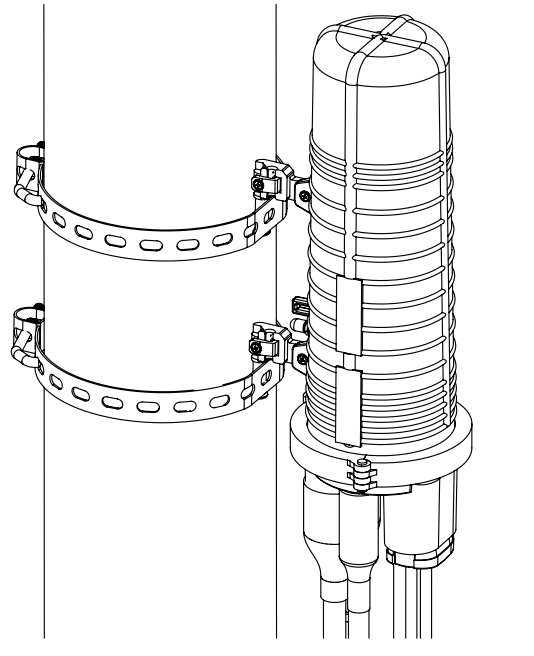
\includegraphics[width=\linewidth]{./images/caixa_emenda_fixacao_em_poste.png}
	\caption{CE fixada em poste}
	\label{fig:ce_fixacao_poste}
  \end{minipage}
  \hfill
  \begin{minipage}[c]{0.6\linewidth}
	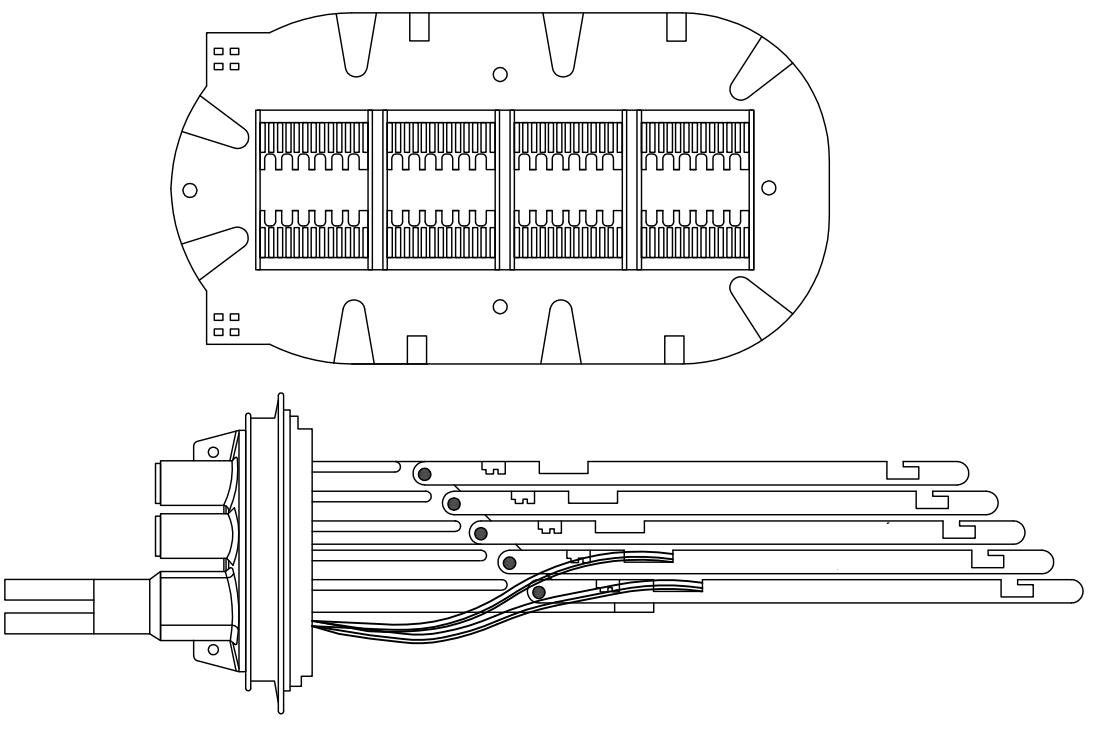
\includegraphics[width=\linewidth]{./images/caixa_emenda_detalhe_bandejas.png}
	\caption{Detalhe das bandejas de CE}
	\label{fig:ce_detalhe_bandejas}
  \end{minipage}
\end{figure}

\subsection{Algoritmos}
O problema de roteamento em redes pode ser resolvido por diferentes algoritmos.
Os mais relevantes para o presente artigo são Dijkstra (encontra o caminho de
menor custo em grafos com pesos não negativos) \cite{dijkstra2022note} e
Bellman-Ford (lida com arestas de peso negativo, mas com maior complexidade
temporal). Para redes ópticas, em que os custos são sempre não negativos
(distância, atenuação, ou custo de instalação), o algoritmo de Dijkstra é mais
adequado.

O roteamento de fibras pode ser formulado como um problema de programação
linear inteira \cite{griva2008linear}, onde variáveis binárias indicam se uma
fibra ou enlace é utilizado. Entretanto, tais problemas são NP-difíceis
\cite{artigorwa}, devido à combinação exponencial de caminhos possíveis. Por
isso, heurísticas como Dijkstra são práticas e eficientes em instâncias reais.

Além da escolha do caminho, a rede precisa alocar espectro e largura de banda.
O problema de \textit{Routing and Wavelength Assignment} (RWA) é conhecido por
sua complexidade computacional, reforçando a necessidade de algoritmos
heurísticos e aproximativos \cite{artigorwa}.

\begin{figure}
  \begin{minipage}[c]{0.45\linewidth}
	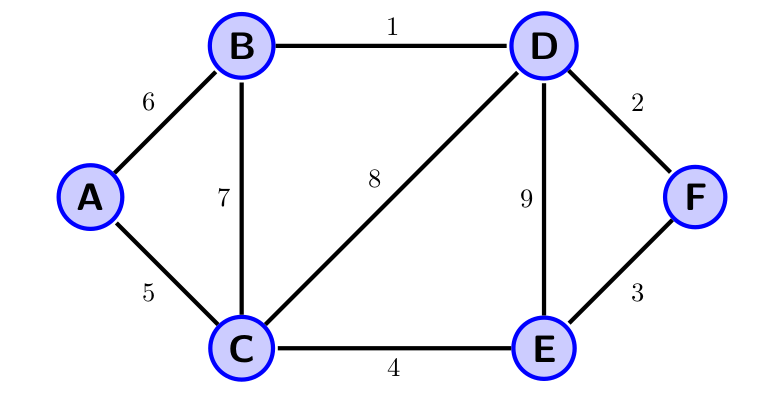
\includegraphics[width=\linewidth]{./images/dijkastra_01.png}
	\caption{Grafo com custos}
	\label{fig:dijkastra_graph}
  \end{minipage}
  \hfill
  \begin{minipage}[c]{0.58\linewidth}
	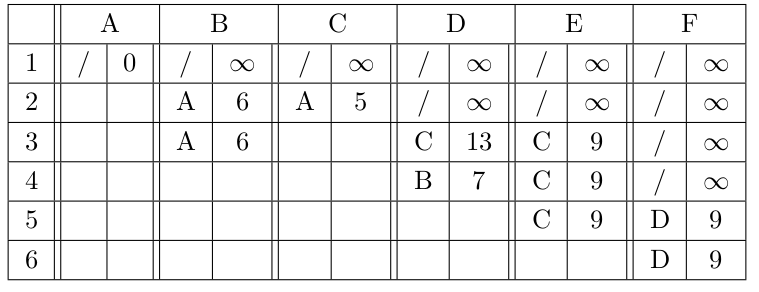
\includegraphics[width=\linewidth]{./images/dijkastra_02.png}
	\caption{Iterações do algoritmo Dijkastra}
	\label{fig:dijkastra_table}
  \end{minipage}
\end{figure}

